\documentclass[ignorenonframetext,xcolor=x11names]{beamer}

\input{../common.preamble.beamer.tex}
 
\title{Business 4720 - Class 8}

\subtitle{Data Visualization with Python}

\begin{document}

\begin{frame}{}
  \titlepage
  \footnotesize
  \input{../license.tex}
\end{frame}

\begin{frame}{This Class}

\begin{block}{What You Will Learn:}
\begin{itemize}
  \item Visualizing data with Python using the Plotly Express library
  \item Interactive data dashboards with Plotly Dash
\end{itemize}
\end{block}
\end{frame}

\begin{frame}{Example Dataset}
\begin{itemize}
  \item Government of Canada, Open Government Portal
  \item Fuel Consumption Ratings -- Battery-electric vehicles -- 2012--2023; last updated Oct 10, 2023
  \item \href{https://open.canada.ca/data/en/dataset/98f1a129-f628-4ce4-b24d-6f16bf24dd64}{https://open.canada.ca/data/en/dataset/98f1a129-f628-4ce4-b24d-6f16bf24dd64}
\end{itemize}
\centering
\footnotesize

	\begin{tabular}{|l|l|} \hline
	  {\bf Column} & {\bf Data Type} \\ \hline \hline
	  Make & Discrete \\ 
	  Model & Discrete \\
	  Year & Numeric \\
	  Category & Discrete \\
	  City & Numeric\footnote{Fuel consumption in l/100km equivalent} \\
	  Hwy & Numeric \\
	  Comb & Numeric \\
	  Range & Numeric\footnote{Range in km} \\ \hline
	\end{tabular}
\end{frame}

\begin{frame}[fragile]{Data Preparation}

Import required packages:

\begin{pythoncode}
import pandas as pd
import plotly.express as px
import plotly.io as pio
pio.kaleido.scope.mathjax = None
\end{pythoncode}

\begin{pythoncode}
# Read data
data = pd.read_csv('https://evermann.ca/busi4720/fuel.csv')
\end{pythoncode}
\end{frame}

\begin{frame}[fragile]{Histogram}
\begin{pythoncode}
# Create histogram
fig = px.histogram(data, x='Range', nbins=50)

# Show histogram, interactive in browser
fig.show()

# Save figure to image
fig.write_image("px.histogram.pdf", height=500, width=750)
\end{pythoncode}
\begin{center}
    \includegraphics[height=2in]{px.histogram.pdf}
\end{center}
\end{frame}

%\begin{frame}[fragile]{Histogram with Summary Information}
%Prepare some summary statistics:

%\footnotesize
%\begin{pythoncode}
%# Calculating summary statistics
%mean_v = fuel['Range'].mean()
%median_v = fuel['Range'].median()
%lower95 = fuel['Range'].quantile(0.025)
%upper95 = fuel['Range'].quantile(0.975)

%# Creating the density plot
%fig = px.histogram(fuel, x='Range', 
         %color_discrete_sequence=['pink'])
%\end{pythoncode}
%\end{frame}

%\begin{frame}[fragile]{Histogram with Summary Information \small [cont'd]}
%\footnotesize
%\begin{pythoncode}
%# Adding vertical lines and annotations
%fig.add_vline(x=mean_v, line_dash='dash', 
      %annotation_text=f'Mean = {round(mean_v)}', 
      %annotation_position='top right')
%fig.add_vline(x=median_v, line_dash='dot', 
      %annotation_text=f'Median = {round(median_v)}', 
      %annotation_position='bottom right')
%fig.add_vline(x=lower95, line_dash='dot', 
      %annotation_text=f'L95 = {round(lower95)}', 
      %annotation_position='top left')
%fig.add_vline(x=upper95, line_dash='dot', 
      %annotation_text=f'U95 = {round(upper95)}', 
      %annotation_position='bottom left')

%fig.update_layout(
    %title='Density Plot - Years 2012 to 2024',
    %xaxis_title='Range (km)',
    %yaxis_title='Proportion of Vehicles')
%\end{pythoncode}
%\end{frame}

%\begin{frame}{Histogram with Summary Information}
    %\includegraphics[width=\textwidth]{px.histogram2.pdf}
%\end{frame}


\begin{frame}[fragile]{Column Chart}
Prepare data in ''long'' format using \texttt{pd.melt()}:
\begin{columns}
\begin{column}{.55\textwidth}
\begin{pythoncode}
data_grouped = \
data.groupby('Year') \
  .agg(
     meanCity=('City','mean'),
     meanHwy=('Hwy','mean')) \
  .reset_index()

data_long = \
  pd.melt(data_grouped, 
      id_vars=['Year'], 
      value_vars=['meanCity', 
                  'meanHwy'], 
      var_name='metric', 
      value_name='consumption')
\end{pythoncode}
\end{column}
\begin{column}{.525\textwidth}
\begin{textcode}
>>> data_grouped
    Year  meanCity   meanHwy
0   2012  2.050000  2.500000
1   2013  2.266667  2.500000
2   2014  2.155556  2.433333
3   2015  2.178571  2.392857
4   2016  2.318519  2.388889
\end{textcode}
\begin{textcode}
>>> data_long
    Year    metric  consumption
0   2012  meanCity     2.050000
1   2013  meanCity     2.266667
2   2014  meanCity     2.155556
3   2015  meanCity     2.178571
4   2016  meanCity     2.318519
\end{textcode}
\end{column}
\end{columns}
\end{frame}

\begin{frame}[fragile]{Column Chart \small [cont'd]}

\begin{pythoncode}
fig = px.bar(data_long, 
   x='Year', y='consumption', color='metric', 
   barmode='group')
\end{pythoncode}
\begin{columns}
\begin{column}{.65\textwidth}
  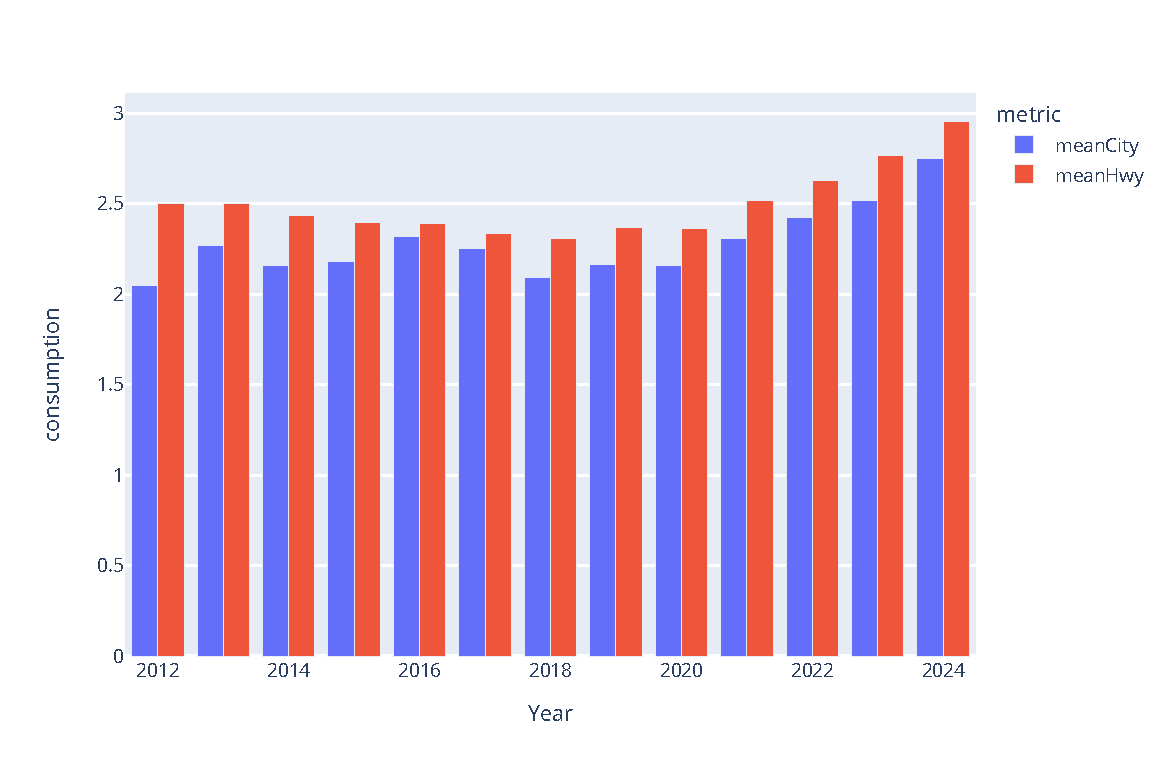
\includegraphics[height=2in]{px.fuel.columns.pdf}
\end{column}
\begin{column}{.35\textwidth}
\footnotesize
  \begin{itemize}
  \item The \texttt{barmode='group'} places bars of different categories next to each other (instead of stacking them)
  \end{itemize}
\end{column}
\end{columns}
\end{frame}


\begin{frame}[fragile]{Labelling}
\begin{pythoncode}
fig = px.bar(data_long,
  x='Year', y='consumption', color='metric', barmode='group',
  text_auto=True,
  title = 'Electric Vehicle Range',
  labels={'consumption': 'Mean Consumption (l/100km)', 
          'Year': 'Calendar Year', 
          'metric': 'Drive Mode'})
\end{pythoncode}
\begin{columns}
\begin{column}{.65\textwidth}
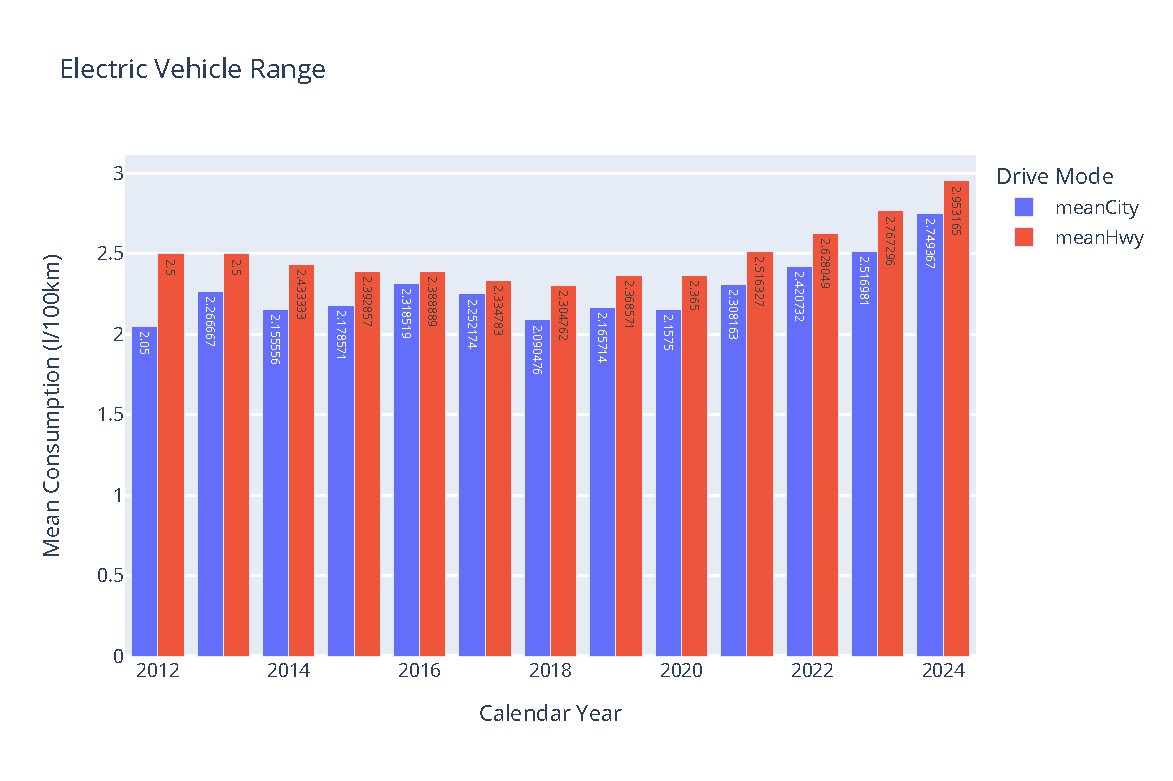
\includegraphics[height=2in]{px.fuel.columns.labels.pdf}
\end{column}
\begin{column}{.35\textwidth}
\footnotesize
  \begin{itemize}
  \item No subtitles or captions
  \item Labels for each plot element
  \item Values with \texttt{text\_auto=True} option
  \end{itemize}
\end{column}
\end{columns}
\end{frame}

\begin{frame}[fragile]{Column Chart (with Patterns)}
\begin{pythoncode}
fig = px.bar(data_long, 
   x='Year', y='consumption', 
   pattern_shape = 'metric', 
   pattern_shape_sequence = ['.', 'x', '+', '|', '-', '/'],
   barmode='group')
\end{pythoncode}
\begin{columns}
\begin{column}{.75\textwidth}
  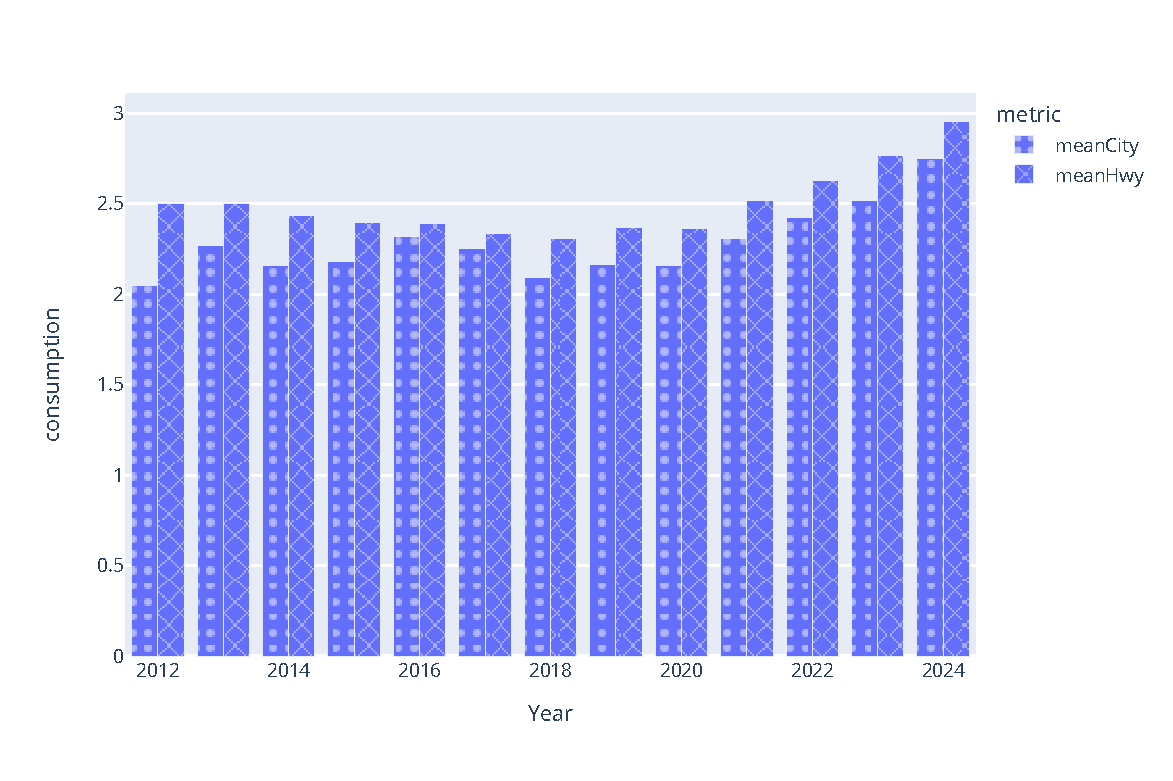
\includegraphics[width=\textwidth]{px.fuel.columnsPatterns.pdf}
\end{column}
\begin{column}{.35\textwidth}
\footnotesize
  \begin{itemize}
  \item Note the different pattern shapes
  \end{itemize}
\end{column}
\end{columns}
\end{frame}

\begin{frame}{Hands-On Exercises}
\begin{block}{}
\begin{enumerate}
    \item Read the EV fuel efficiency data set into a Pandas data frame.
    \item Create a histogram of highway fuel efficiency with 25 bins.
    \item Add labels for the axes, and add a title.
\end{enumerate}
\end{block}

\begin{block}{Tips}
    \begin{itemize} 
       \item Use the \texttt{pd.read\_csv()} function from Pandas
       \item The column name is \texttt{Hwy}
       \item Use the \texttt{px.histogram()} function from Plotly Express
       \item Use the \texttt{title=\ldots} option
       \item Use the \texttt{labels='\ldots'} option
    \end{itemize}
\end{block}
\end{frame}


\begin{frame}[fragile]{Box Plot}
\begin{pythoncode}
data_long = pd.melt(data, 
    id_vars=['Year'], value_vars=['City', 'Hwy'], 
    var_name='metric', value_name='consumption')
fig = px.box(data_long, 
             x='Year', y='consumption', color='metric')
\end{pythoncode}
\begin{columns}
\begin{column}{.75\textwidth}
  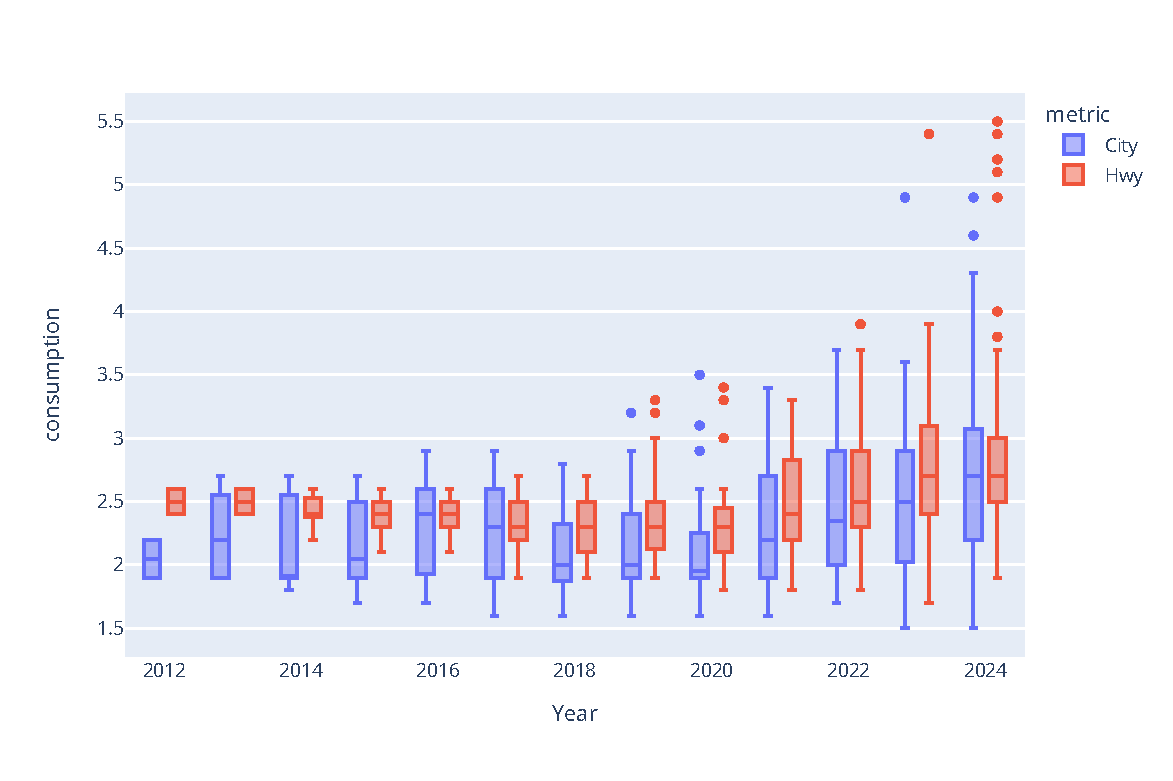
\includegraphics[width=\textwidth]{px.fuel.box.pdf}
\end{column}
\begin{column}{.35\textwidth}
\footnotesize
\begin{itemize}
   \item Shows distribution
   \item Median
   \item 1st quartile $Q_1$
   \item 3rd quartile $Q_3$
   \item ''Inter-quartile range''
   \item $IQR = Q_3 - Q_1$
   \item ''Whiskers''
   \item $Q_3 + 1.5 \times IQR$
   \item $Q_1 - 1.5 \times IQR$
   \item ''Outliers''
\end{itemize}
\end{column}
\end{columns}
\end{frame}

\begin{frame}[fragile]{Violin Plot}
\footnotesize
\begin{pythoncode}
data_long = pd.melt(data, 
    id_vars=['Year'], value_vars=['City', 'Hwy'], 
    var_name='metric', value_name='consumption')
fig = px.violin(data_long, 
                x='Year', y='consumption', color='metric')
\end{pythoncode}
\begin{columns}
\begin{column}{.75\textwidth}
  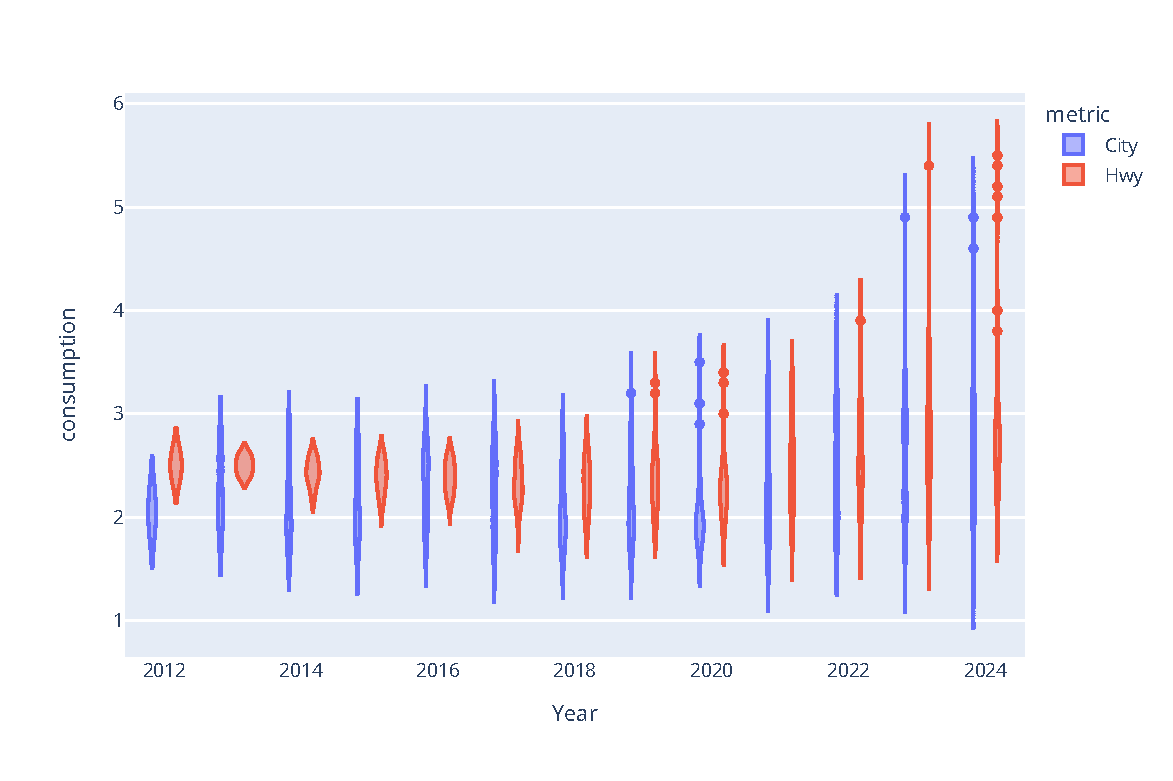
\includegraphics[width=\textwidth]{px.fuel.violin.pdf}
\end{column}
\begin{column}{.35\textwidth}
\footnotesize
\begin{itemize}
   \item Shows detailed density
   \item But no summary statistics
\end{itemize}
\end{column}
\end{columns}
\end{frame}

\begin{frame}[fragile]{Count Plot}
\footnotesize
\begin{pythoncode}
count_data = data \
   .groupby(['Year', 'Category']) \
   .agg(counts = ('Range', 'size')) \
   .reset_index()

fig = px.scatter(count_data, x='Year', y='Category', size='counts')
\end{pythoncode}
\begin{center}
  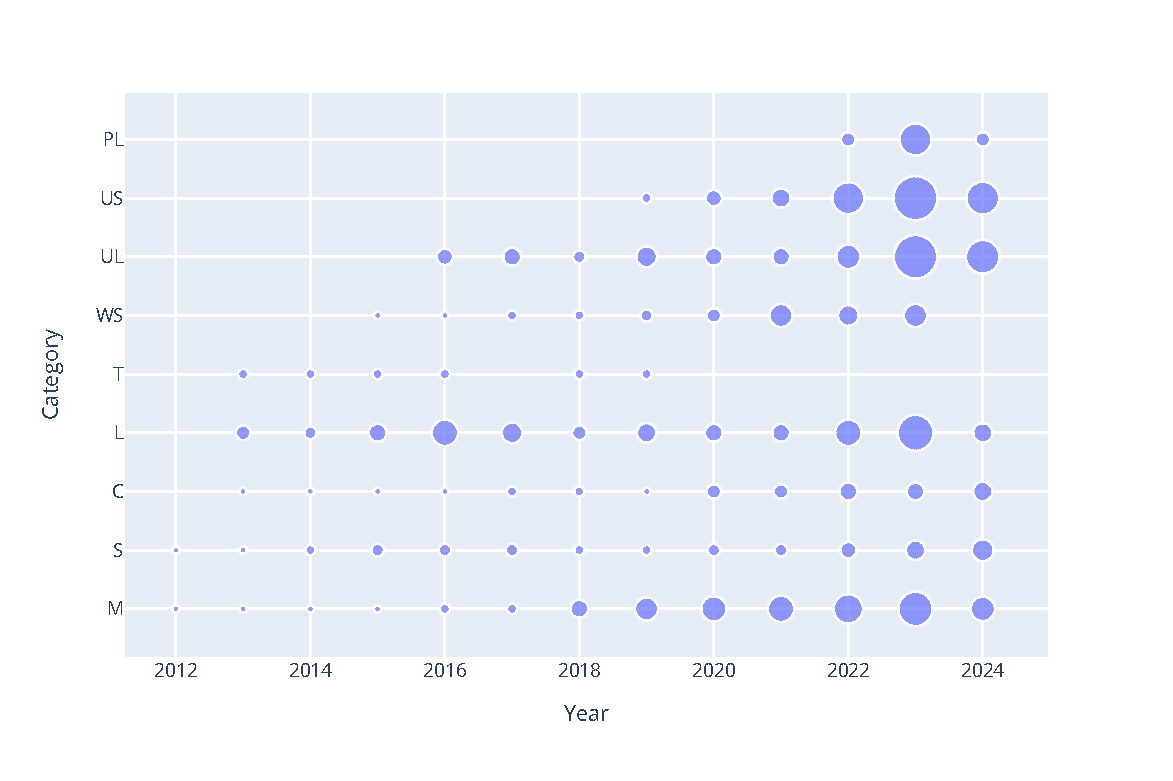
\includegraphics[height=2in]{px.fuel.count.pdf}
\end{center}
\end{frame}

\begin{frame}[fragile]{Points Plot}
\footnotesize
\begin{pythoncode}
grouped_data = data \
    .groupby(['Year', 'Category']) \
    .agg(totalcount=('Range', 'size'),
         meanRange=('Range', 'mean')) \
    .reset_index()
fig = px.scatter(grouped_data, 
           x='Year', y='meanRange', 
           size='totalcount', color='Category')
\end{pythoncode}
\begin{columns}
\begin{column}{.65\textwidth}
  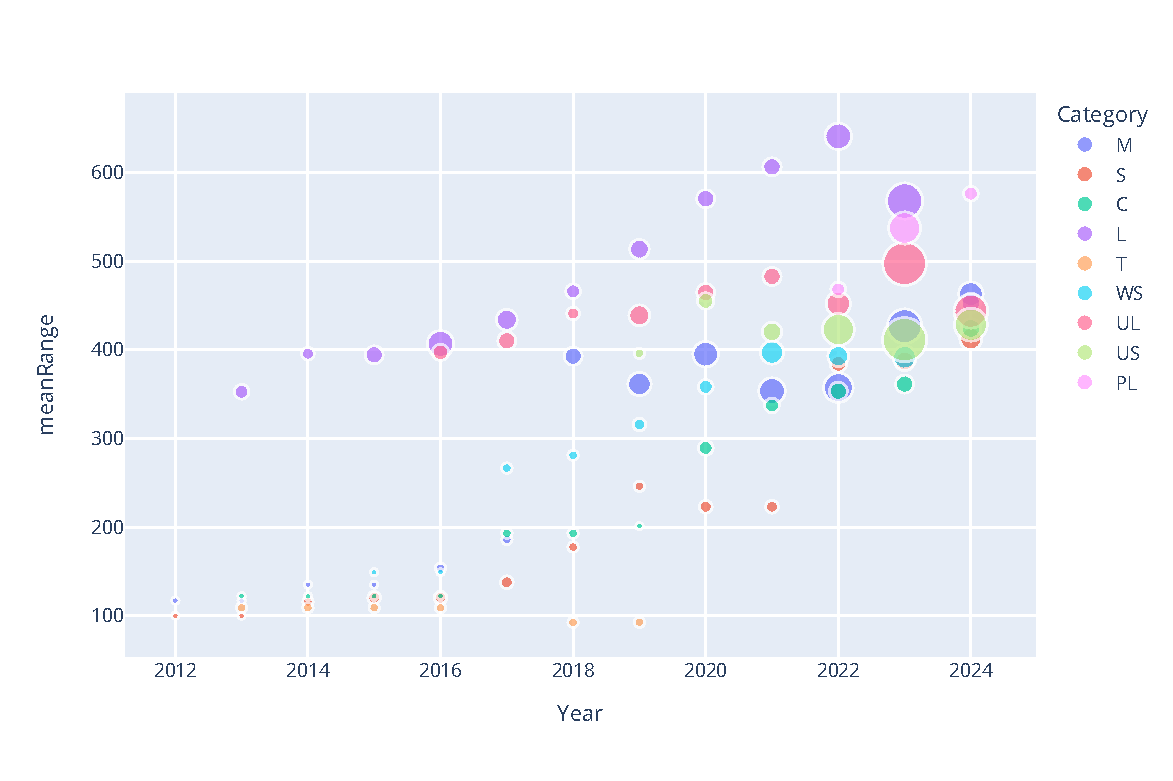
\includegraphics[height=1.75in]{px.fuel.pointsSize.pdf}
\end{column}
\begin{column}{.35\textwidth}
\footnotesize
\begin{itemize}
   \item Shows 4 variables
\end{itemize}
\end{column}
\end{columns}
\end{frame}


\begin{frame}[fragile]{Lines and Points Plot}
\footnotesize
\begin{pythoncode}
filtered_data = 
    data.groupby(['Year', 'Category']) \
       .agg(meanRange=('Range', 'mean')) \
       .reset_index() \
       [data['Category'].isin(['C','L','M','S','US','UL'])] 
fig = px.line(filtered_data, 
    x='Year', y='meanRange', color='Category', 
    symbol='Category', markers=True)
\end{pythoncode}
\begin{columns}
\begin{column}{.65\textwidth}
  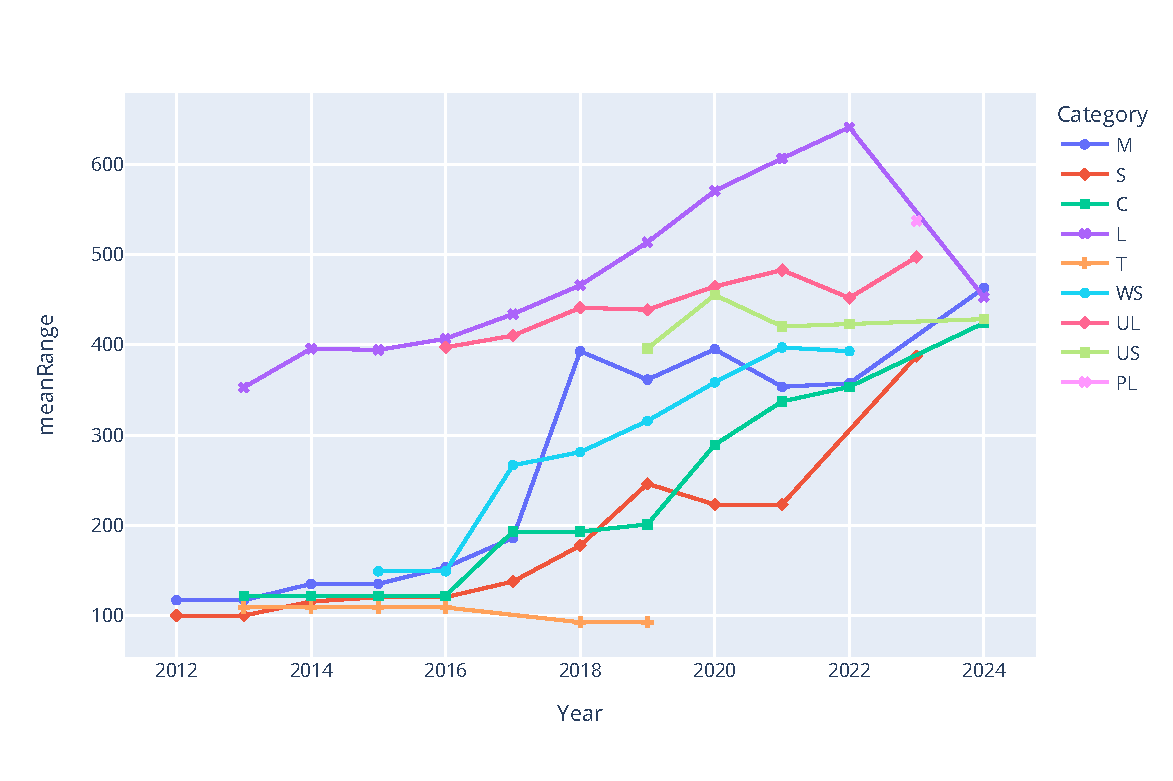
\includegraphics[width=\textwidth]{px.fuel.linesPoints.pdf}
\end{column}
\begin{column}{.35\textwidth}
\footnotesize
\begin{itemize}
   \item Category mapped to two plot elements
\end{itemize}
\end{column}
\end{columns}
\end{frame}


\begin{frame}[fragile]{Pie/Donut Chart}
\begin{columns}
\begin{column}{.6\textwidth}
\begin{pythoncode}
data_pie = \
  data[data['Year'] == 2023] \
    .groupby('Make') \
    .agg(totalcount=('Model', 'size')) \
    .reset_index() \
    .query('totalcount >= 5')

fig = px.pie(data_pie, 
    names='Make', 
    values='totalcount', 
    hole=0.4)
\end{pythoncode}
\end{column}
\begin{column}{.55\textwidth}
  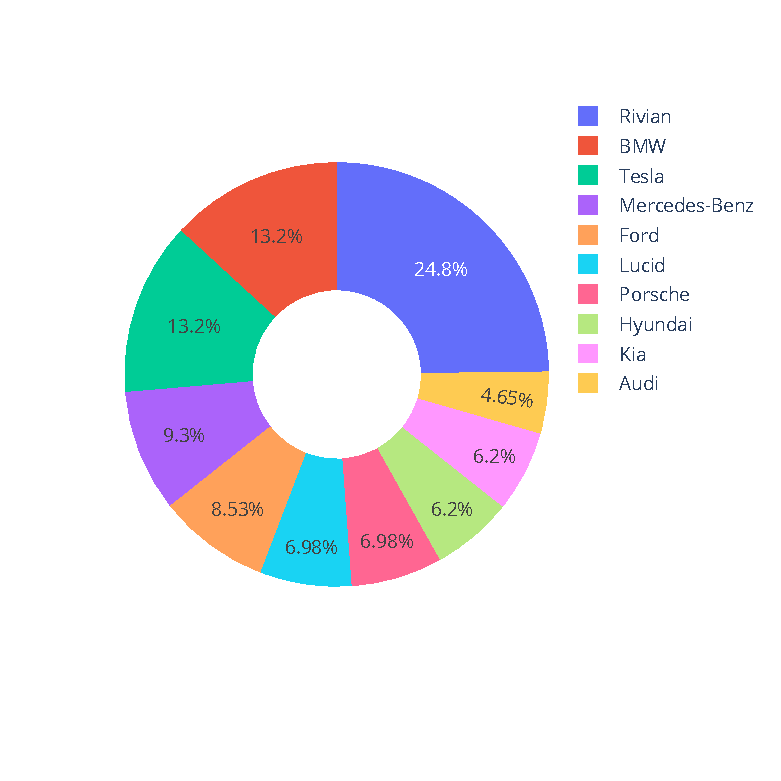
\includegraphics[width=\textwidth]{px.fuel.donut.pdf}
\end{column}
\end{columns}
\end{frame}

%\begin{frame}[fragile]{Donut Chart}
%\footnotesize
%\begin{pythoncode}
%fig = px.pie(fuel_grouped, 
    %names='Make', values='totalcount', hole=0.4,
    %title='EV Offerings by Make (2023, >= 5 models)',
    %labels={'totalcount': 'Number of Models'})
%\end{pythoncode}
%\end{frame}

%\begin{frame}{Pie Chart}
%\centering
  %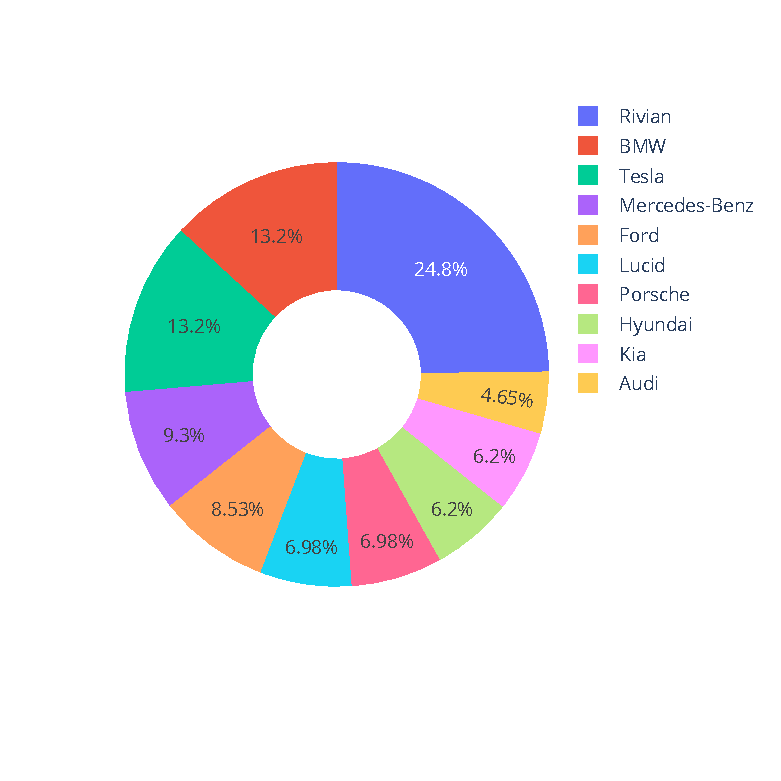
\includegraphics[width=.8\textwidth]{px.fuel.donut.pdf}
%\end{frame}


\begin{frame}[fragile]{Radar Plot}
\begin{columns}
\begin{column}{.67\textwidth}
\begin{pythoncode}
from sklearn.preprocessing \
  import MinMaxScaler
grouped = data \
  .query('Year == 2023') \
  .groupby('Make') \
  .agg(
    Cty=('City',lambda x: 1/x.mean()),
    Hwy=('Hwy',lambda x: 1/x.mean()),
    Rng=('Range',lambda x: x.mean()/100),
    nModels=('Make','size')) \
  .query('nModels >= 5')
grouped[['Cty', 'Hwy', 'Rng']] = \
  MinMaxScaler().fit_transform(
    grouped[['Cty', 'Hwy', 'Rng']])
melted = grouped \
  .reset_index() \
  .melt(id_vars='Make', 
    value_vars=['Cty', 'Hwy', 'Rng'])
fig = px.line_polar(melted, 
     r='value', theta='variable', 
     color='Make', 
     line_close=True)
\end{pythoncode}
\end{column}
\begin{column}{.5\textwidth}
  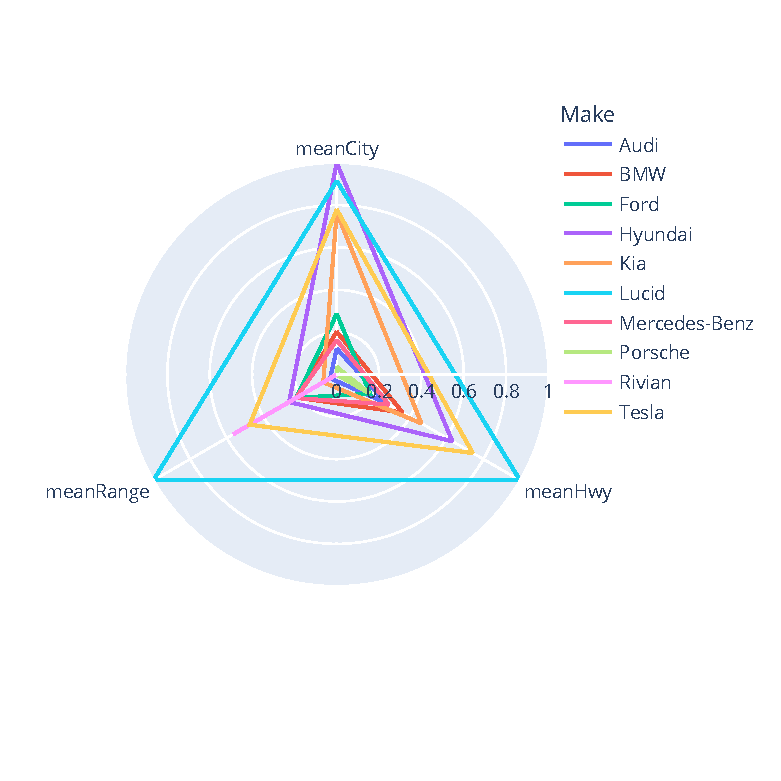
\includegraphics[width=\textwidth]{px.fuel.radar.pdf}
  \end{column}
\end{columns}
\end{frame}


\begin{frame}[fragile]{Local Regression Smoothing Plot}
\begin{pythoncode}
fig = px.scatter(data, 
    x='City', y='Hwy', 
    trendline='lowess',
    trendline_color_override='red')
\end{pythoncode}
\begin{columns}
\begin{column}{.65\textwidth}
  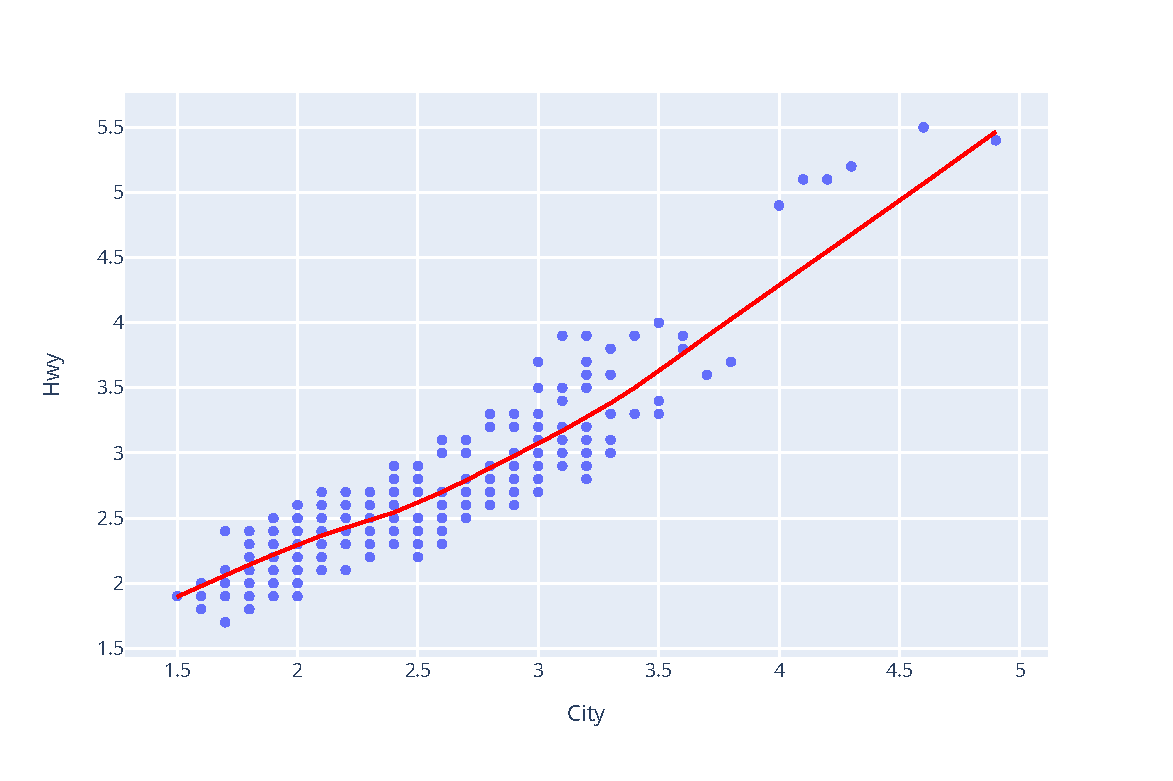
\includegraphics[height=2in]{px.fuel.linesSmooth.pdf}
\end{column}
\begin{column}{.35\textwidth}
\footnotesize
  \begin{itemize}
     \item Local regression line
   \end{itemize}
\end{column}
\end{columns}
\end{frame}


\begin{frame}[fragile]{2D Histogram Plot}
\footnotesize
\begin{pythoncode}
import plotly.graph_objects as go

fig = px.scatter(data, x='Hwy', y='City')

fig.add_trace(
  go.Histogram2dContour(x=data['Hwy'], y=data['City']))
\end{pythoncode}
\begin{columns}
\begin{column}{.65\textwidth}
  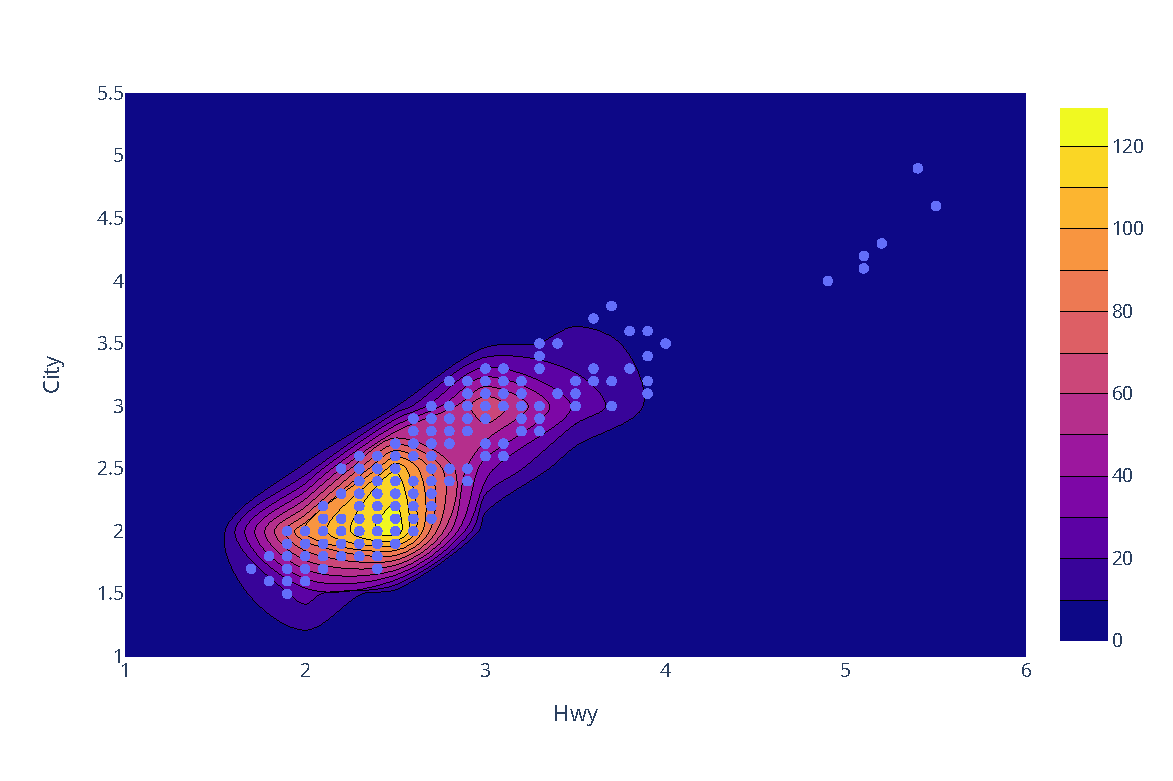
\includegraphics[height=2in]{px.fuel.density2d.pdf}
\end{column}
\begin{column}{.35\textwidth}
\footnotesize
  \begin{itemize}
     \item Counts of observations/data points
   \end{itemize}
\end{column}
\end{columns}
\end{frame}

\begin{frame}[fragile]{Density Heatmap with Marginals}
\scriptsize
\begin{pythoncode}
fig = px.density_heatmap(data,
  x = 'City', y = 'Hwy',
  nbinsx=20, nbinsy=20,
  marginal_x='histogram', marginal_y='histogram',
  color_continuous_scale = px.colors.sequential.Viridis)
\end{pythoncode}
\begin{columns}
\begin{column}{.65\textwidth}
  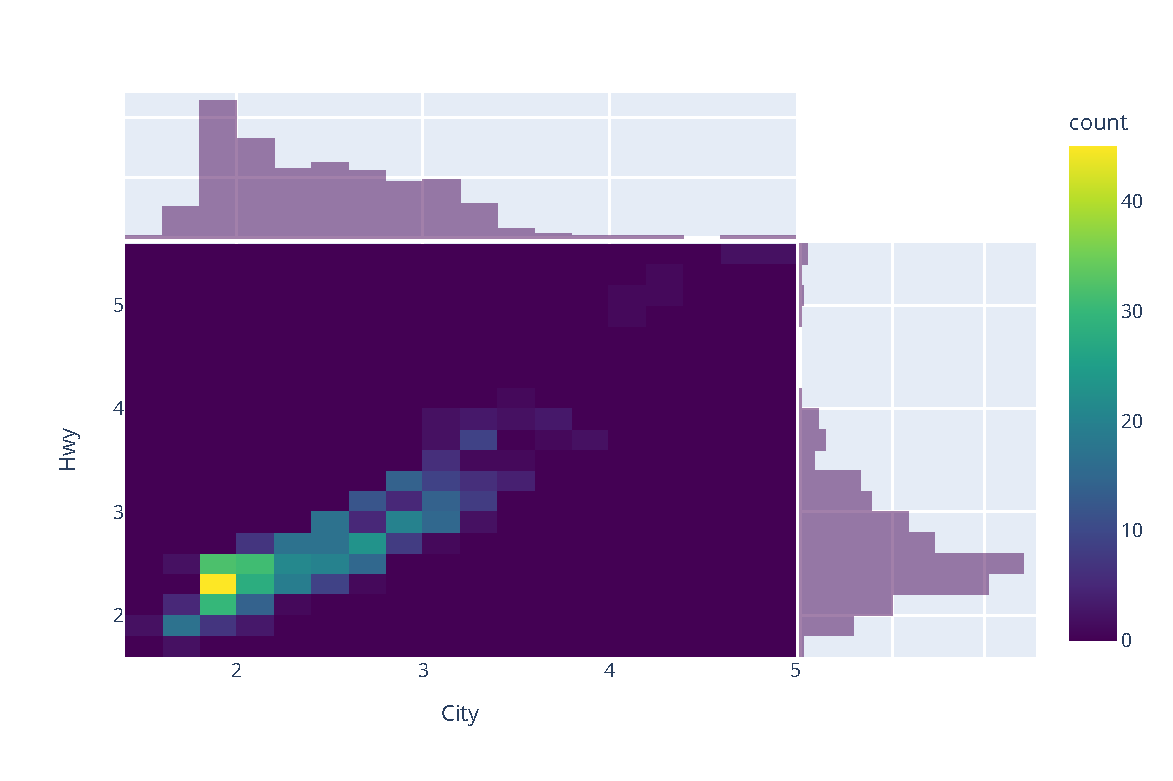
\includegraphics[height=2in]{px.heatmap.pdf}
\end{column}
\begin{column}{.35\textwidth}
\footnotesize
  \begin{itemize}
     \item Marginals can be applied to other plot types
     \item Other options for the marginal plots are \texttt{rug}, \texttt{box}, and \texttt{violin}.
     \item Custom colour palette/scale
   \end{itemize}
\end{column}
\end{columns}
\end{frame}

\begin{frame}{Dashboards}
\begin{columns}
\begin{column}{.35\textwidth}
\footnotesize
\begin{itemize}
   \item Set of related plots
   \item Interactive and customizable
   \item Automatically updated
   \item Simple and easy to understand
   \item Provides quick overview of key metrics
\end{itemize}
\end{column}
\begin{column}{.65\textwidth}
  \includegraphics[width=\textwidth]{px.dash.screenshot.png}
\end{column}
\end{columns}
\end{frame}

\begin{frame}[fragile]{Step 1 -- Import Packages}

\begin{pythoncode}
from dash import Dash, html, dcc, callback, Output, Input
import dash_bootstrap_components as dbc

import plotly.express as px
\end{pythoncode}
\end{frame}

\begin{frame}[fragile]{Step 2 -- Visual Layout}
\begin{itemize}
  \item Container element with multiple Row elements
  \item Row elements contain Column elements, HTML elements, Label elements, Selection elements, Radio button elements, etc.
\end{itemize}
\begin{center}
  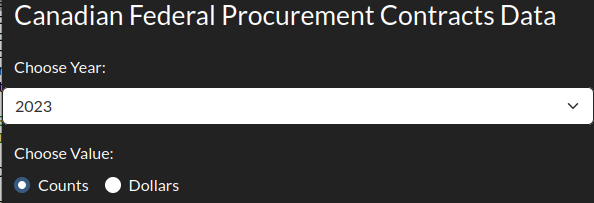
\includegraphics[width=.6\textwidth]{dashboard1.png}
\end{center}
\begin{itemize}
  \item First row is HTML heading
  \item Second row is Label element and Selection element, followed by another Label element and Radio button element
\end{itemize}
\end{frame}
\end{frame}

\begin{frame}[fragile]{Step 2 -- Visual Layout \small [cont'd]}
\begin{pythoncode}
app.layout = dbc.Container([
  dbc.Row([
    html.H3('Canadian Federal Procurement Contracts Data')]),
  dbc.Row([
    html.P(),
    dbc.Label('Choose Year: '),
    dbc.Select(
      id='year-selection',
      options=[{"label": x, "value": x} for x in years],
      value=years[-1]),
    html.P(),
    dbc.Label('Choose Value: '),
    dbc.RadioItems(
      options=[{"label": "Counts", "value": 0},
               {"label": "Dollars", "value": 1}],
      value=0, inline = True,
      id = 'value-selection'),
    html.P() ]),
\end{pythoncode}
\vspace{-\baselineskip}
\begin{itemize}
  \item Every component has an ID!
\end{itemize}
\end{frame}

\begin{frame}{Step 2 -- Visual Layout \small [cont'd]}
\begin{center}
  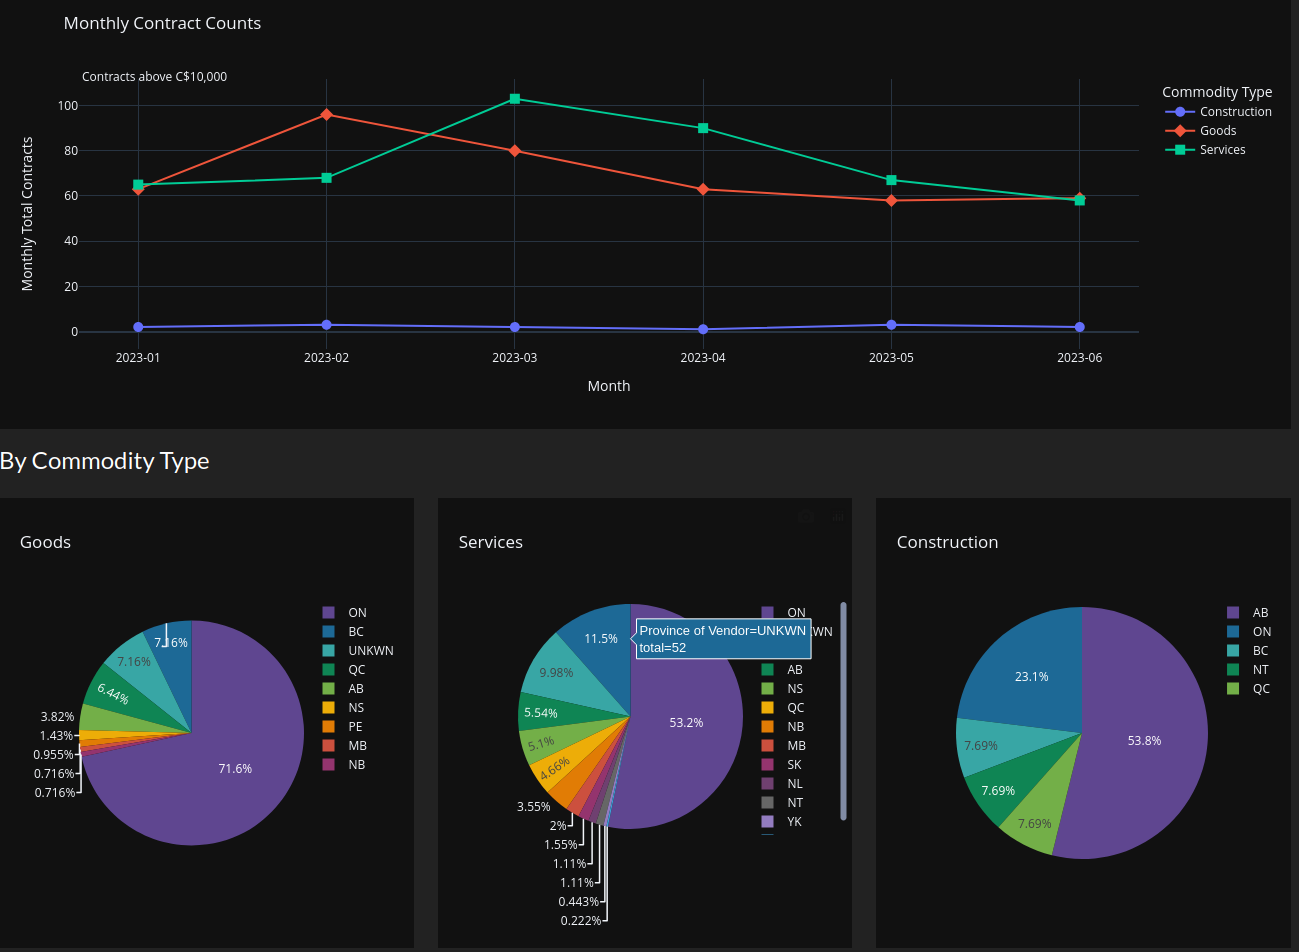
\includegraphics[width=.6\textwidth]{dashboard2.png}
\end{center}
\small
\begin{itemize}
  \item First row contains single column with a Graph element that contains a figure (line chart)
  \item Second row is an HTML heading
  \item Third row contains three columns, each with one graph element that contain a figure (pie chart)
\end{itemize}
\end{frame}

\begin{frame}[fragile]{Step 2 -- Visual Layout \small [cont'd]}
\begin{pythoncode}
# Continued from previous snippet
   dbc.Row([
        dbc.Col([
            dcc.Graph(figure={}, id='line')
        ], width=12),
    ]),
    dbc.Row([
        html.P(),
        html.H4('By Commodity Type'),
        html.P()
    ]),
    dbc.Row([
        dbc.Col([
            dcc.Graph(figure={}, id='pie1')
        ], width=4),
        dbc.Col([
            dcc.Graph(figure={}, id='pie2')
        ], width=4),
        dbc.Col([
            dcc.Graph(figure={}, id='pie3')
        ], width=4),
    ]),
\end{pythoncode}
\end{frame}

\begin{frame}[fragile]{Step 3 -- Create the Figures}
\begin{pythoncode}
@callback(
    Output(component_id='line', component_property='figure'),
    [
        Input(component_id='year-selection', 
              component_property='value'),
        Input(component_id='value-selection', 
              component_property='value')
    ]
)
def update_line(year_chosen, value_chosen): 
    # Figure creation code, for example
    # fig = px.histogram(...)
    return fig
\end{pythoncode}
\footnotesize
\begin{itemize}
   \item Each figure has an update function that creates and returns the figure
   \item Each update function has a callback specification
   \begin{itemize}
   \footnotesize
      \item The \texttt{Output} specifies the Graph element for this figure
      \item The \texttt{Input} elements specify which interactive elements provide values for creating or updating the figure
   \end{itemize}
\end{itemize}
\end{frame}

\begin{frame}[fragile]{Step 4 -- Run the App}

\begin{pythoncode}
app.run()
\end{pythoncode}
\end{frame}

\begin{frame}{Hands-On Exercises}
\footnotesize
Use the Pagila film rentals data from \url{https://evermann.ca/busi4720/rentals.csv}
\begin{enumerate}
   \item Read the data into a Pandas data frame using \texttt{read\_csv()}
   \item Create a box plot of the rental payment amounts for films by rating
   \item Create a violin plot of the rental payment amounts for films by rating
\end{enumerate}
\begin{itemize}
\item Compare the information conveyed by a box plot and a violin plot. What are the commonalities and what are the differences?
\end{itemize}
\end{frame}

\begin{frame}{Hands-On Exercises}

\footnotesize
Use the Pagila film rentals data from \url{https://evermann.ca/busi4720/rentals.csv}
\begin{enumerate}
   \item Read the data into a Pandas data frame using \texttt{read\_csv()}
   \item Use \texttt{drop\_duplicates()} to drop duplicates of the film titles
   \begin{itemize}
      \item Because each film may have been rented multiple times.
   \end{itemize}
   \item Produce a \emph{histogram} of counts of films by rating
\end{enumerate}
\vspace{\baselineskip}
\textbf{Tip:}
\begin{itemize}
\item Use the \texttt{columns} and \texttt{shape} properties or the \texttt{describe()} method of a data frame to examine it. 
\end{itemize}
\end{frame}

\begin{frame}{Hands-On Exercises}

\footnotesize
Use the Pagila film rentals data from \url{https://evermann.ca/busi4720/rentals.csv}
\begin{enumerate}
   \item Read the data into a Pandas data frame using \texttt{read\_csv()}
   \item Create a data frame with the mean rental payments for films by rating
   \item Generate a bar chart of the mean rental payments for films by rating
   \item Generate a pie or donut chart of rental counts by film rating
\end{enumerate}

\vspace{\baselineskip}
\textbf{Tips:}
\begin{itemize}
   \item Use the \texttt{groupby()} function to group the data
   \item Use the \texttt{mean()} and \texttt{std()} to find the mean and standard deviation of for a data frame column
\end{itemize}
\end{frame}


\end{document}
